
\begin{figure}[t]
\centering
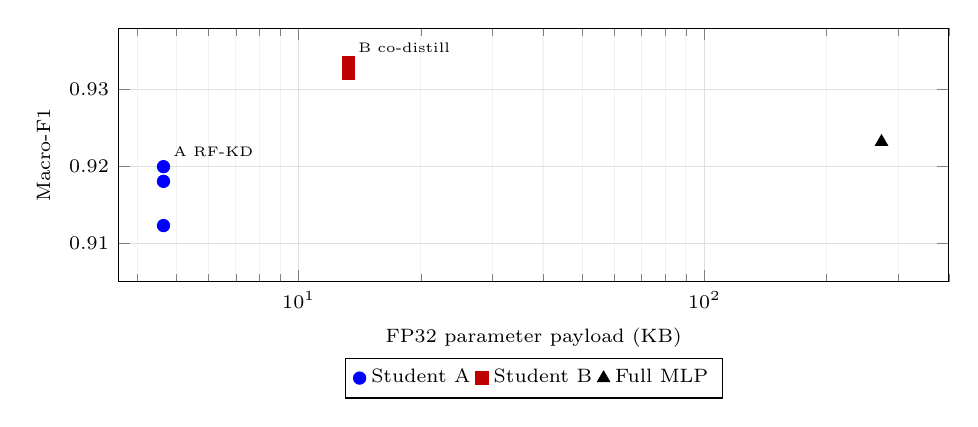
\begin{tikzpicture}
\begin{axis}[
  width=\columnwidth,height=48mm,
  xmode=log,log basis x=10,
  xmin=3.6,xmax=400,ymin=0.905,ymax=0.938,
  xlabel={FP32 parameter payload (KB)},ylabel={Macro-F1},
  grid=both,major grid style={gray!25},minor grid style={gray!10},
  legend style={font=\scriptsize,at={(0.5,-0.30)},anchor=north,legend columns=3},
  tick label style={font=\scriptsize},label style={font=\scriptsize}
]
\addplot[only marks,mark=*,mark size=2.2pt,blue] coordinates {
 (4.64453,0.912303)
 (4.64453,0.919971)
 (4.64453,0.918062) };
\addlegendentry{Student A}
\addplot[only marks,mark=square*,mark size=2.2pt,red!75!black] coordinates {
 (13.26953,0.932169)
 (13.26953,0.932808)
 (13.26953,0.933526) };
\addlegendentry{Student B}
\addplot[only marks,mark=triangle*,mark size=2.5pt,black] coordinates {
 (273.01953,0.923195) };
\addlegendentry{Full MLP}
\node[font=\tiny,anchor=south west] at (axis cs:4.6445,0.919971) {A RF-KD};
\node[font=\tiny,anchor=south west] at (axis cs:13.2695,0.933526) {B co-distill};
\end{axis}
\end{tikzpicture}
\caption{WSN-DS size--performance trade-off. Points are ten-seed means; all configurations at a student capacity share the same FP32 parameter size.}
\label{fig:wsn-tradeoff}
\end{figure}
